\documentclass[12pt]{article}

\title{Activity 3: Data Types}
\author{Dr. Chris Mayfield}
\date{CS 149, Fall 2016}

%\ProvidesPackage{cspogil}

% fonts
\usepackage[utf8]{inputenc}
\usepackage[T1]{fontenc}
\usepackage{mathpazo}

% spacing
\usepackage[margin=2cm]{geometry}
\renewcommand{\arraystretch}{1.4}
\setlength{\parindent}{0pt}

% orphans and widows
\clubpenalty=10000
\widowpenalty=10000
\pagestyle{empty}

% figures and tables
\usepackage{graphicx}
\usepackage{multicol}
\usepackage{tabularx}
\usepackage{wrapfig}

% fixed-width columns
\usepackage{array}
\newcolumntype{L}[1]{>{\raggedright\let\newline\\\arraybackslash\hspace{0pt}}m{#1}}
\newcolumntype{C}[1]{>{\centering\let\newline\\\arraybackslash\hspace{0pt}}m{#1}}
\newcolumntype{R}[1]{>{\raggedleft\let\newline\\\arraybackslash\hspace{0pt}}m{#1}}

% include paths
\makeatletter
\def\input@path{{Models/}{../../Models/}}
\graphicspath{{Models/}{../../Models/}}
\makeatother

% colors
\usepackage[svgnames,table]{xcolor}
\definecolor{bgcolor}{HTML}{FAFAFA}
\definecolor{comment}{HTML}{007C00}
\definecolor{keyword}{HTML}{0000FF}
\definecolor{strings}{HTML}{B20000}

% table headers
\newcommand{\tr}{\bf\cellcolor{Yellow!10}}

% syntax highlighting
\usepackage{textcomp}
\usepackage{listings}
\lstset{
    basicstyle=\ttfamily\color{black},
    backgroundcolor=\color{bgcolor},
    numberstyle=\scriptsize\color{comment},
    commentstyle=\color{comment},
    keywordstyle=\color{keyword},
    stringstyle=\color{strings},
    columns=fullflexible,
    keepspaces=true,
    showlines=true,
    showstringspaces=false,
    upquote=true
}

% code environments
\newcommand{\java}[1]{\lstinline[language=java]{#1}}%[
\lstnewenvironment{javalst}{\lstset{language=java,backgroundcolor=}}{}
\lstnewenvironment{javabox}{\lstset{language=java,frame=single,numbers=left}\quote}{\endquote}

% PDF properties
\usepackage[pdftex]{hyperref}
\urlstyle{same}
\makeatletter
\hypersetup{
  pdftitle={\@title},
  pdfauthor={\@author},
  pdfsubject={\@date},
  pdfkeywords={},
  bookmarksopen=false,
  colorlinks=true,
  citecolor=black,
  filecolor=black,
  linkcolor=black,
  urlcolor=blue
}
\makeatother

% titles
\makeatletter
\renewcommand{\maketitle}{\begin{center}\LARGE\@title\end{center}}
\makeatother

% boxes [optional height]
\newcommand{\emptybox}[1][10em]{
\vspace{1em}
\begin{tabularx}{\linewidth}{|X|}
\hline\\[#1]\hline
\end{tabularx}}

% models
\newcommand{\model}[1]{\section{#1}\nopagebreak}
\renewcommand{\thesection}{Model~\arabic{section}}

% questions
\newcommand{\quest}[1]{\subsection*{Questions~ (#1)}}
\newcounter{question}
\newcommand{\Q}{\vspace{1em}\refstepcounter{question}\arabic{question}.~ }
\renewcommand{\thequestion}{\#\arabic{question}}

% sub-question lists
\usepackage{enumitem}
\setenumerate[1]{label=\alph*)}
\setlist{itemsep=1em,after=\vspace{1ex}}

% inline answers
\definecolor{answers}{HTML}{C0C0C0}
\newcommand{\ans}[1]{%
\ifdefined\Student
    \leavevmode\phantom{~~\textcolor{answers}{#1}}
\else
    ~~\textcolor{answers}{#1}
\fi}

% longer answers [optional height]
\newsavebox{\ansbox}
\newenvironment{answer}[1][4em]{
\nopagebreak
\begin{lrbox}{\ansbox}
\begin{minipage}[t][#1]{\linewidth}
\color{answers}
}{
\end{minipage}
\end{lrbox}
\ifdefined\Student
    \phantom{\usebox{\ansbox}}%
\else
    \usebox{\ansbox}%
\fi}


\begin{document}

\maketitle

Java supports two main types of data: \emph{primitive types} like \java{int} and \java{double} that represent a single value, and \emph{reference types} like \java{String} and \java{Scanner} that represent more complex information.

% Based on Model 2 of "Activity 01 - Operators" by Helen Hu

\model{The \% Operator}

\vspace{-1ex}
\begin{center}
\begin{tabular}[t]{|C{35pt}|C{65pt}|C{35pt}|}
\hline
 9 / 4 & \textit{evaluates to} & 2 \\
\hline
10 / 4 & \textit{evaluates to} & 2 \\
\hline
11 / 4 & \textit{evaluates to} & 2 \\
\hline
12 / 4 & \textit{evaluates to} & 3 \\
\hline
13 / 4 & \textit{evaluates to} & 3 \\
\hline
14 / 4 & \textit{evaluates to} & 3 \\
\hline
15 / 4 & \textit{evaluates to} & 3 \\
\hline
16 / 4 & \textit{evaluates to} & 4 \\
\hline
\end{tabular}
\hspace{0.5in}
\begin{tabular}[t]{|C{35pt}|C{65pt}|C{35pt}|}
\hline
 9 \% 4 & \textit{evaluates to} & 1 \\
\hline
10 \% 4 & \textit{evaluates to} & 2 \\
\hline
11 \% 4 & \textit{evaluates to} & 3 \\
\hline
12 \% 4 & \textit{evaluates to} & 0 \\
\hline
13 \% 4 & \textit{evaluates to} & 1 \\
\hline
14 \% 4 & \textit{evaluates to} & 2 \\
\hline
15 \% 4 & \textit{evaluates to} & 3 \\
\hline
16 \% 4 & \textit{evaluates to} & 0 \\
\hline
\end{tabular}
\end{center}


\quest{15 min}


\Q Which numbers \% 4 evaluate to 0 in the table above?
If the table were extended to include more rows, which other numbers \% 4 would evaluate to 0?

\begin{answer}
12 and 16. Other numbers include 0, 4, 8, 20, 24.
\end{answer}


\Q Look at the expressions in the second table that evaluate to 1.
How do the left operands in these expressions (9, 13, 17) differ from those that evaluate to 0?

\begin{answer}
They differ by one.
\end{answer}


\Q List three numbers \% 5 that will evaluate to 0 and three numbers \% 5 that will evaluate to 2.

\begin{answer}
0, 5, 10 and 2, 7, 12.
\end{answer}


\Q Evaluate the following Java expressions:

\begin{center}
\begin{tabular}{C{1in}C{1in}C{1in}C{1in}}
18 \% 4 \ans{= ~2} &
19 \% 4 \ans{= ~3} &
19 \% 5 \ans{= ~4} &
19 \% 6 \ans{= ~1} \\
\end{tabular}
\end{center}


\Q Consider how you were taught to do long division in elementary school.
Finish solving for $79 \div 5$.
What is the answer?

\begin{center}
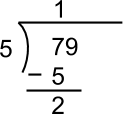
\includegraphics[scale=0.65]{div79by5.png}
\end{center}

\begin{answer}[3em]
We first bring the 9 down, then 5 goes into 29 five times, and so we subtract 25. The final answer is 15 remainder 4.
\end{answer}


\Q Imagine that you are given candy mints to divide evenly among your team members.

\begin{enumerate}
\item If your team receives 11 mints, how many mints are left over?

\ans{\java{11 \% 4} is 3 ~~or~~ \java{11 \% 5} is 1}

\item If your team receives 2 mints, how many mints are left over?

\ans{\java{2 \% 4} is 2 ~~or~~ \java{2 \% 5} is 2}
\end{enumerate}


\Q Describe what the \% operator does.
How are the / and \% operators related?

\begin{answer}
Both operators divide two numbers: \% returns the remainder, and / returns the quotient.
\end{answer}


\Q Would it make sense to apply the \% operator to real numbers?
Why or why not?

\begin{answer}
Not really, since the concept of remainder is based on integer division.

(BTW floating-point modulo is defined in IEEE 754, but its use is rare.)
\end{answer}

\model{Primitive Types}
\label{CS1/primitive-types}

\vspace{-1ex}
\begin{table}[h!]
\begin{tabularx}{\linewidth}{|X|X|X|X|}
\hline
\tr Keyword    & \tr Size & \tr Min Value & \tr Max Value \\
\hline
\java{byte}    & 1 byte   & $-128$    & $127$ \\
\hline
\java{short}   & 2 bytes  & $-32,768$ & $32,767$ \\
\hline
\java{int}     & 4 bytes  & $-2^{31}$ & $2^{31}-1$ \\
\hline
\java{long}    & 8 bytes  & $-2^{63}$ & $2^{63}-1$ \\
\hline
\java{float}   & 4 bytes  & $\pm 3.4 \times 10^{-38}$  & $\pm 3.4 \times 10^{38}$ \\
\hline
\java{double}  & 8 bytes  & $\pm 1.7 \times 10^{-308}$ & $\pm 1.7 \times 10^{308}$ \\
\hline
\java{boolean} & N/A      & \java{false}     & \java{true} \\
\hline
\java{char}    & 2 bytes  & \java{'\\u0000'} & \java{'\\uffff'} \\
\hline
\end{tabularx}
\end{table}

Note that 1 byte is 8 bits, i.e., eight ``ones and zeros'' in computer memory.
Since there are only two options for each bit, with 8 bits you can represent $2^8 = 256$ possible values.


\quest{10 min}


\Q Which of the primitive types are integers? Which are floating-point? Which are not numeric?

\begin{answer}
\end{answer}


\Q Why do primitive types have ranges of values? What determines the range of the data type?

\begin{answer}
\end{answer}


\Q Why can't computers represent every possible number in mathematics? Will they ever be able to do so?

\begin{answer}
\end{answer}


\Q Since a \java{byte} can represent 256 different numbers, why is its max value 127 and not 128?

\begin{answer}
\end{answer}


\Q What is the data type for each of the following values?

\begin{quote}
\begin{multicols}{2}
1.14159 \ans{double} \\[1ex]
0       \ans{int} \\[1ex]
-1.0F   \ans{float} \\[1ex]
123     \ans{int}

7.2E-4  \ans{double} \\[1ex]
0.0     \ans{double} \\[1ex]
-13L    \ans{long} \\[1ex]
'0'     \ans{char}
\end{multicols}
\end{quote}


\Q Given the following variable declarations, which of the assignments are not allowed?

\begin{quote}
\begin{multicols}{2}

\begin{javalst}
byte miles;
short minutes;
int checking;
long days;
float total;
double sum;
boolean flag;
char letter;
\end{javalst}

\begin{javalst}
checking = 56000;
total = 0;
sum = total;
total = sum;
checking = miles;
sum = checking;
sum = days;
days = "0";
\end{javalst}

\end{multicols}
\end{quote}


\Q \label{allow} In general, when does Java allow you to assign one type of numeric variable to another?

\begin{answer}
\end{answer}


\Q Based on your answer to \ref{allow}, list all possible assignments in this format:
\java{int} $\gets$ \java{short}

\begin{answer}
\end{answer}

\model{Reference Types}

\begin{quote}
\begin{minipage}{0.5\linewidth}

\begin{javalst}
int count;
double price;
String name;
Scanner in;

count = 0;
price = 1.99;
name = "Beyonce";
in = new Scanner(System.in);
\end{javalst}

\end{minipage}
\begin{minipage}{0.5\linewidth}

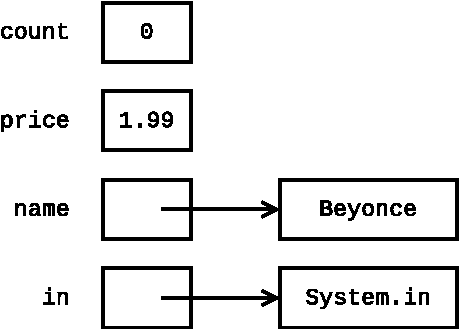
\includegraphics{CS1/reference1.pdf}

\end{minipage}
\end{quote}

Java has eight primitive types (see \ref{CS1/primitive-types}).
All other types of data are called \emph{reference} types, because \textbf{their value is a memory address}.
When drawing memory diagrams, use an arrow to \emph{reference} other memory locations (rather than make up integer values for the actual addresses).


\quest{10 min}


\Q What are the reference types in the example above?

\begin{answer}
\end{answer}


\Q In terms of style, what is the difference between primitive and reference type names?

\begin{answer}
\end{answer}


\Q Variables in Java can use at most eight bytes of memory. Explain why the values for Beyonce and System.in cannot be stored directly in the memory cells for \java{name} and \java{in}.

\begin{answer}
\end{answer}


\Q What is the value of the variable \java{count}? What is the value of the variable \java{price}?

\begin{answer}
\end{answer}


\Q What is the value of the variable \java{name}? What is the value of the variable \java{in}?

\begin{answer}
\end{answer}


\Q \label{assign} Carefully explain what it means to assign one variable to another. For example, what does the statement ~ \java{price = count;}~ do in terms of memory?

\begin{answer}
\end{answer}


\Q Draw a memory diagram for the following code. Make sure your answer is consistent with what you wrote for \ref{assign}.

\begin{javalst}
int width;
float score;
String first;
Scanner input;
String other;

width = 20;
score = 0.94;
first = "Taylor";
input = new Scanner(System.in);
score = width;
other = first;
\end{javalst}


\end{document}
